%%%%%%%%%%%%%%%%%%%%%%%%%%%%%%%%%%%%%%%%%%%%%%%%%%%%%%%%%%%%%%%%%
%%%%%%%%%%                                             %%%%%%%%%%
%%%%%%%%%%  You can reuse this work under:             %%%%%%%%%%
%%%%%%%%%%  CC-BY-4.0 OR  etalab-2.0                   %%%%%%%%%%
%%%%%%%%%%                                             %%%%%%%%%%
%%%%%%%%%%  Henri Bretel, Delphine Le Piolet,          %%%%%%%%%%
%%%%%%%%%%  Laili Rahimie, Romain Thomas ; 2025        %%%%%%%%%%
%%%%%%%%%%                                             %%%%%%%%%%
%%%%%%%%%%  science.ouverte@universite-paris-saclay.fr %%%%%%%%%%
%%%%%%%%%%  DiBISO - Université Paris-Saclay           %%%%%%%%%%
%%%%%%%%%%                                             %%%%%%%%%%
%%%%%%%%%%%%%%%%%%%%%%%%%%%%%%%%%%%%%%%%%%%%%%%%%%%%%%%%%%%%%%%%%


%% needed for the template to find the class dir when the class folder
%% is not stored in the same directory than the main tex file
%\def\classdir{dibiso}

\newcommand{\reportyear}{2024}
\newcommand{\halcollectionid}{UNIV-PARIS-SACLAY}
\newcommand{\labacronym}{UPSaclay}
\newcommand{\labfullname}{Université Paris-Saclay}
\newcommand{\datafetchdate}{24/09/2025}
\newcommand{\watermarktext}{}

\newcommand{\anrprojectsinfo}{Le nombre d'entités affichées a été limité à 20. Dans l'API, 1637 entités ont été trouvées.\\}
\newcommand{\chaptersinfo}{}
\newcommand{\collaborationsnb}{2957}
\newcommand{\institutionsnb}{1269}
\newcommand{\countriesnb}{82}
\newcommand{\collaborationmapworldinfo}{\emoji{warning} Le traitement des données a été limité par le nombre maximal d'entités téléchargeables (1000). Des données peuvent être manquantes ou les valeurs peuvent être inférieures aux valeurs réelles. \\}
\newcommand{\collaborationmapeuropeinfo}{\emoji{warning} Le traitement des données a été limité par le nombre maximal d'entités téléchargeables (1000). Des données peuvent être manquantes ou les valeurs peuvent être inférieures aux valeurs réelles. \\}
\newcommand{\collaborationnamesinfo}{Le nombre d'entités affichées a été limité à 40. Dans l'API, 14322 entités ont été trouvées.\\}
\newcommand{\conferencesinfo}{Le nombre d'entités affichées a été limité à 40. Dans l'API, 2609 entités ont été trouvées.\\}
\newcommand{\europeanprojectsinfo}{Le nombre d'entités affichées a été limité à 20. Dans l'API, 551 entités ont été trouvées.\\}
\newcommand{\bsojournalsnbworks}{1000}
\newcommand{\bsojournalsnbworksfoundinbso}{792}
\newcommand{\bsojournalsnbjournals}{503}
\newcommand{\bsojournalsbsoversion}{2024Q4}
\newcommand{\journalsinfo}{\emoji{warning} Le traitement des données a été limité par le nombre maximal d'entités téléchargeables (1000). Des données peuvent être manquantes ou les valeurs peuvent être inférieures aux valeurs réelles. \\}
\newcommand{\journalshalinfo}{Le nombre d'entités affichées a été limité à 40. Dans l'API, 3407 entités ont été trouvées.\\}
\newcommand{\oaworksperiod}{2020 - 2024}
\newcommand{\openaccessworksinfo}{}
\newcommand{\privatesectorcollaborationsinfo}{\emoji{warning} Le traitement des données a été limité par le nombre maximal d'entités téléchargeables (1000). Des données peuvent être manquantes ou les valeurs peuvent être inférieures aux valeurs réelles. \\}
\newcommand{\workstypeinfo}{}



\documentclass[french, 11pt]{dibiso/biso}
\usepackage{tikzpagenodes} % For accessing text area coordinates
\usepackage[absolute,overlay]{textpos}

\title{Bilan \\ Science \\ Ouverte}

\author{Direction des bibliothèques, de l'information et de la science ouverte}

\date{Année \reportyear}

\subtitle{\textbf{Laboratoire \labacronym} \\
  \medskip
  \labfullname
}

%\titledescription{}

% Écriver votre nom entre les crochets ci-dessous, par exemple :
% \reporter{Prénom Nom}
\reporter{}
% Écriver votre adresse email entre les crochets ci-dessous, par exemple : 
% \reporteremail{reporter.email@example.com}
\reporteremail{}


%%%%%%%%%%%%%%%%%%%%%%%%%%% COMMENT REMPLIR LE BISO %%%%%%%%%%%%%%%%%%%%%%%%%%%
%                                                                             %
% Commenter des parties à exclure :                                           %
% Pour commenter des sections que vous ne souhaitez pas inclure dans le       %
% rapport final, vous pouvez utiliser le symbole % au début de chaque ligne   %
% que vous souhaitez exclure. Cela peut vous servir à ne pas afficher des     %
% sections du rapports que vous ne jugez pas appropriées pour le laboratoire. %
%                                                                             %
%                                                                             %
% Créer une liste à puces :                                                   %
% Pour créer une liste à puces, utilisez l'environnement itemize. Voici un    %
% exemple :                                                                   %
% \begin{itemize}                                                             %
%     \item Premier élément de la liste                                       %
%     \item Deuxième élément de la liste                                      %
%     \item Troisième élément de la liste                                     %
% \end{itemize}                                                               %
%                                                                             %
%                                                                             % 
% Mettre du texte en gras :                                                   %
% Pour mettre du texte en gras, utilisez la commande \textbf{}. Par exemple : %
% Voici un exemple de \textbf{texte en gras}.                                 %
%                                                                             %
%%%%%%%%%%%%%%%%%%%%%%%%%%% COMMENT REMPLIR LE BISO %%%%%%%%%%%%%%%%%%%%%%%%%%%


\begin{document}

\renewcommand{\arraystretch}{2}


\maketitle

\tableofcontents

\pagebreak



\section{Introduction}


\subsection*{Méthodologie et objectifs}

Le BiSO est un bilan science ouverte établi à partir des publications présentes dans HAL. Il est produit sur l'année $\mathrm{n} - 1$ à l'automne afin de permettre une plus grande exhaustivité des dépôts référencés dans la collection HAL du laboratoire.

Cette démarche est encouragée par la politique Science Ouverte de l'Université\footnote{\url{https://www.universite-paris-saclay.fr/recherche/science-ouverte/la-science-ouverte-luniversite-paris-saclay}} : \\
\say{Objectif n°1 : Faire du libre accès la règle pour l'ensemble des publications scientifiques de l'Université.}

Sauf mention particulière, les données utilisées pour les graphiques proviennent de la collection HAL \texttt{\halcollectionid} et de l'année {\reportyear}.

\subsection*{Calendrier annuel}

\begin{enumerate}
  \item Printemps : Le Référent recherche SO envoie une liste\footnote{Extraction des données avec l'outil \say{HAL Collection checker} : \url{https://simple-hcc-ui.streamlit.app/}} des publications manquantes dans HAL au DU du laboratoire.
  \item Été : les chercheurs et doctorants sont invités à déposer les publications manquantes\footnote{Attention : les publications non renseignées dans HAL ne sont pas incluses dans ce rapport.} dans HAL, idéalement en déposant le texte intégral (version postprint) ou à défaut les notices bibliographiques.
  \item Automne : votre référent recherche produit le BiSO et le communique au DU du laboratoire.
\end{enumerate}


Ce bilan est proposé pour donner un aperçu annuel des atouts SO du laboratoire, en présentant une liste exhaustive des revues, conférences, collaborations et taux d'accès ouvert accompagné d'un relevé des actions en faveur de la science ouverte, et de propositions d'amélioration.

Ce document est à l'attention des directeurs, directrices, et toute personne du laboratoire qui participe activement aux actions de développement de la Science Ouverte. Communiqué seulement en interne, il permet aux référents recherche de vous présenter des données HAL, préalablement nettoyées, avec la participation des chercheurs pour les dépôts, afin de refléter au mieux la production scientifique. Remis chaque année, le BiSO vise également à vous aider à anticiper la préparation de rapports (ex : HCERES).


\subsection*{Déposer dans une archive ouverte}

La loi pour la République Numérique permet aux auteurs travaillant dans une institution publique en France depuis 2016, de partager le postprint sur HAL, avec un embargo de 6 mois pour les disciplines STM et 1 an pour les SHS.

\pagebreak

\section{Liste des revues}


\begin{figure}[!h]
  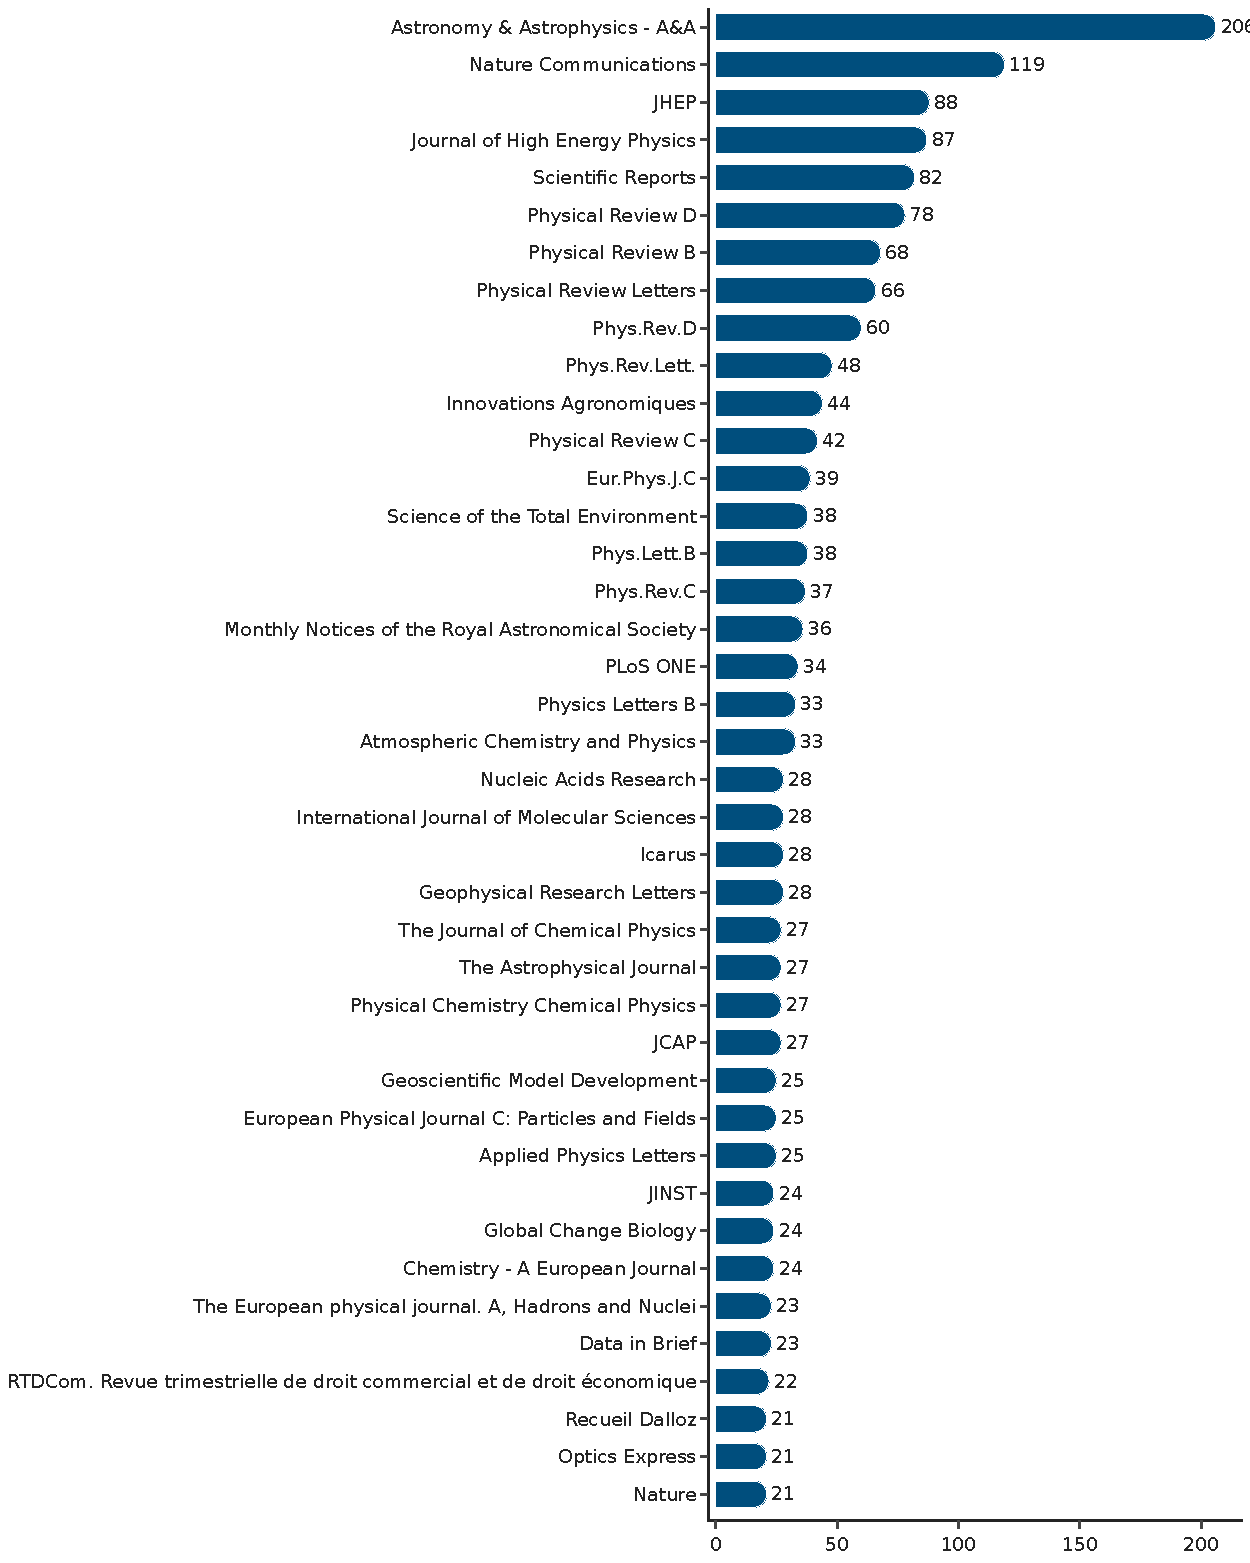
\includegraphics[width=\textwidth]{figures/journals_hal.pdf}
  \centering
  \caption{Revues renseignées dans HAL}
  \label{fig_jorunals_hal}
\end{figure}

{\footnotesize\journalshalinfo}


% Ecrire un commentaire sur la liste des revues dans HAL ci-dessous :





% Fin de la liste des revues dans HAL

\pagebreak

\section{Liste des conférences}

\begin{figure}[!h]
  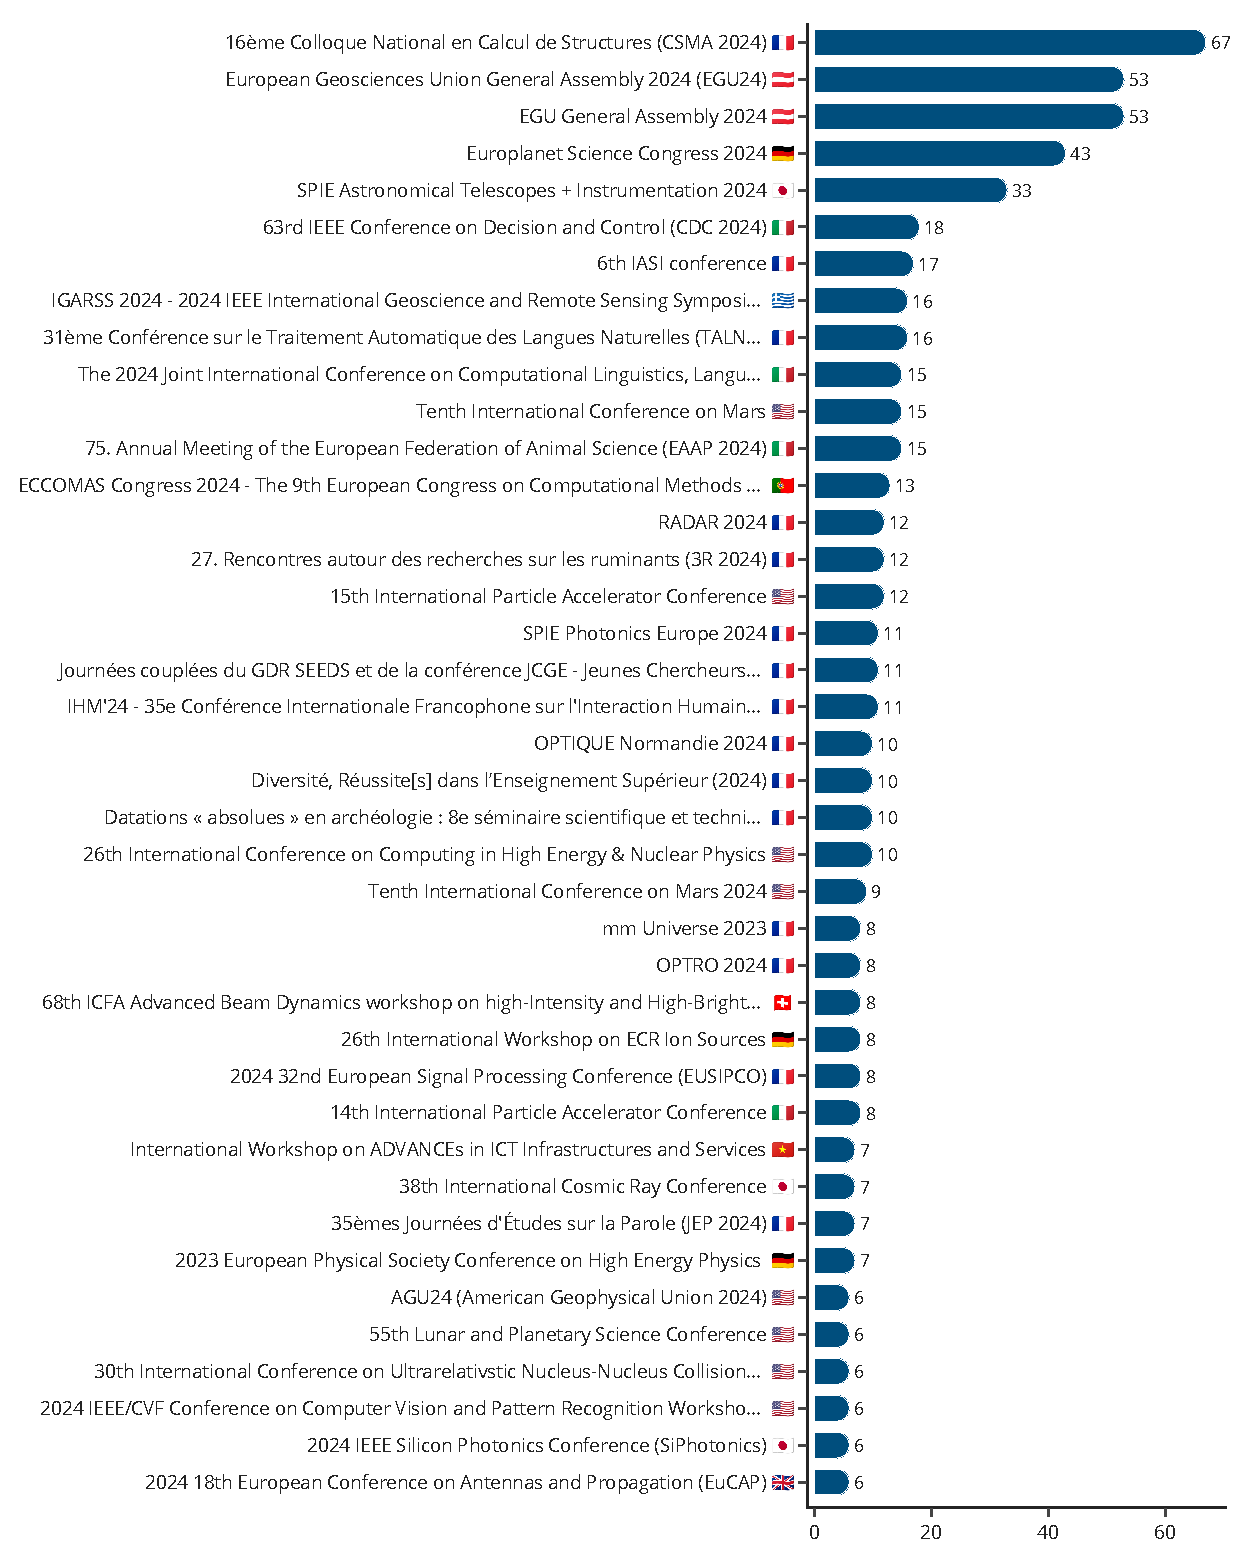
\includegraphics[width=\textwidth]{figures/conferences.pdf}
  \centering
  \caption{Conférences renseignées dans HAL}
  \label{fig_conferences}
\end{figure}

{\footnotesize\conferencesinfo}

\pagebreak

\section{Liste des chapitres}

{
  \footnotesize
  \begin{longtable}{p{.4\linewidth}p{.35\linewidth}p{.15\linewidth}}
\caption{Liste des chapitres renseignés dans HAL}
\label{tab_chapters}\\
\toprule
Titre du chapitre & Titre du livre & Éditeur \\
\midrule
L'agriculture a-t-elle sa place en ville ? & "Ressources" n°6, la revue INRAE &  \\
Die Medien: Schlachten der Kommunikation & Springer eBooks &  \\
Under the ICSU Umbrella: The Joint Commission on Radioactivity (1947-1955) between IUPAP and IUPAC & Globalizing Physics. One Hundred Years of the International Union of Pure and Applied Physics & Oxford University Press \\
Struggles Over the Definition of a “Job Well Done” & Encyclopedia of Professionalization: Organization of Professions, Production of Professionalities and Growth of Professionalism & Wiley \\
Scientific workflows management with blockchain: a survey & Blockchain and smart-contract technologies for innovative applications & Springer Cham \\
Guerre froide : Relations avec des physiciens soviétiques & Les sciences en guerre froide (1946-1991) — France — Union soviétique et pays de l'Est — Témoignages - (coordinateur Claude Debru) & Presses universitaires Rhin \& Danube \\
Some réminiscences & Les sciences en guerre froide (coordinateur: Claude Debru) &  \\
Metallo-β-lactamases & Metalloenzymes & Elsevier \\
L'économie sociale et solidaire : antitode ou excipient du néolibéralisme ? Quelques réflexions à partir du monde associatif & (Re)penser l'économie sociale et solidaire. Approches et historiographie & L'Arbre bleu \\
Transformations de la fonction RH & Ressources Humaines - 4ème édition & Dunod \\
Du dancing à la scène : le jazz dans les casinos de Vichy & Martin Guerpin et Etienne Jardin (dir.) Faites vos jeux ! La vie musicale dans les casinos français (19e-21e siècle) &  \\
Entre Alger et Lunéville. Récits de santé d’une famille bourgeoise & L’orientalisme en train de se faire & EHESS \\
« Les reconversions empêchées des ex-salariés de Renault Billancourt », in Emmanuel de Lescure, Nicolas Divert, Fabienne Maillard, , Rennes, Presses Universitaires de Rennes, 2024. & La formation continue au service de la reconversion ? Les liens fragiles entre aspirations et mobilités dans le monde du travail &  \\
ICT externalities: measurement issues and their effects on output growth & Intangible assets, productivity and economic growth : micro, meso and macro perspectives & Routledge \\
A Conference For Africa. Racialization and the New World Order & The Paris Peace Conference of 1919: The Challenge of a New World Order & Berghahn Books \\
Les frères Basset ou les voies diverses de la colonisation & L’orientalisme en train de se faire & EHESS \\
Les modèles constitutionnels anglais et américain dans l’historiographie constitutionnelle comparée du XIXe siècle & Historiographies constitutionnelles et identités nationales (sous la coordination de Jacky Hummel) & Mare \& Martin \\
Conseil constitutionnel, 14 avril 2023, n° 2023-849, Loi de financement de la sécurité sociale pour 2023 & Les grandes décisions de la jurisprudence constitutionnelle. Approche politique & LGDJ \\
Le nouveau service de l'Etat. Sociologie des régulateurs français & Le moment régulateur. Naissance d'une contre-culture de gouvernement & Presses de Sciences Po \\
Semiparametric estimation in elliptical distributions & Elliptically Symmetric Distributions in Signal Processing and Machine Learning &  \\
Physics-based output-feedback consensus-formation control of networked autonomous vehicles & Hybrid and Networked Dynamical Systems & Springer Verlag \\
Introduction générale : Faire des finances syndicales un objet de recherche & Les finances syndicales & Septentrion \\
L'anthropologie des historiens & Histinéraires. La fabrique de l’histoire telle qu’elle se raconte. Une enquête sur les historiens contemporains &  \\
Ouvertures & Enquêter sur ce qui se passe. Mélanges offerts à Antoine Hennion & Presses des Mines \\
Des inégalités et injustices climatiques à la transition juste ? & Les sociétés face aux défis climatiques : que sait-on ? & CNRS Editions \\
\textbf{Seulement 25 lignes affichées sur 496.} \\
\bottomrule
\end{longtable}

}

{\footnotesize\chaptersinfo}

\pagebreak

\section{Typologie de la production scientifique}

\begin{figure}[!h]
  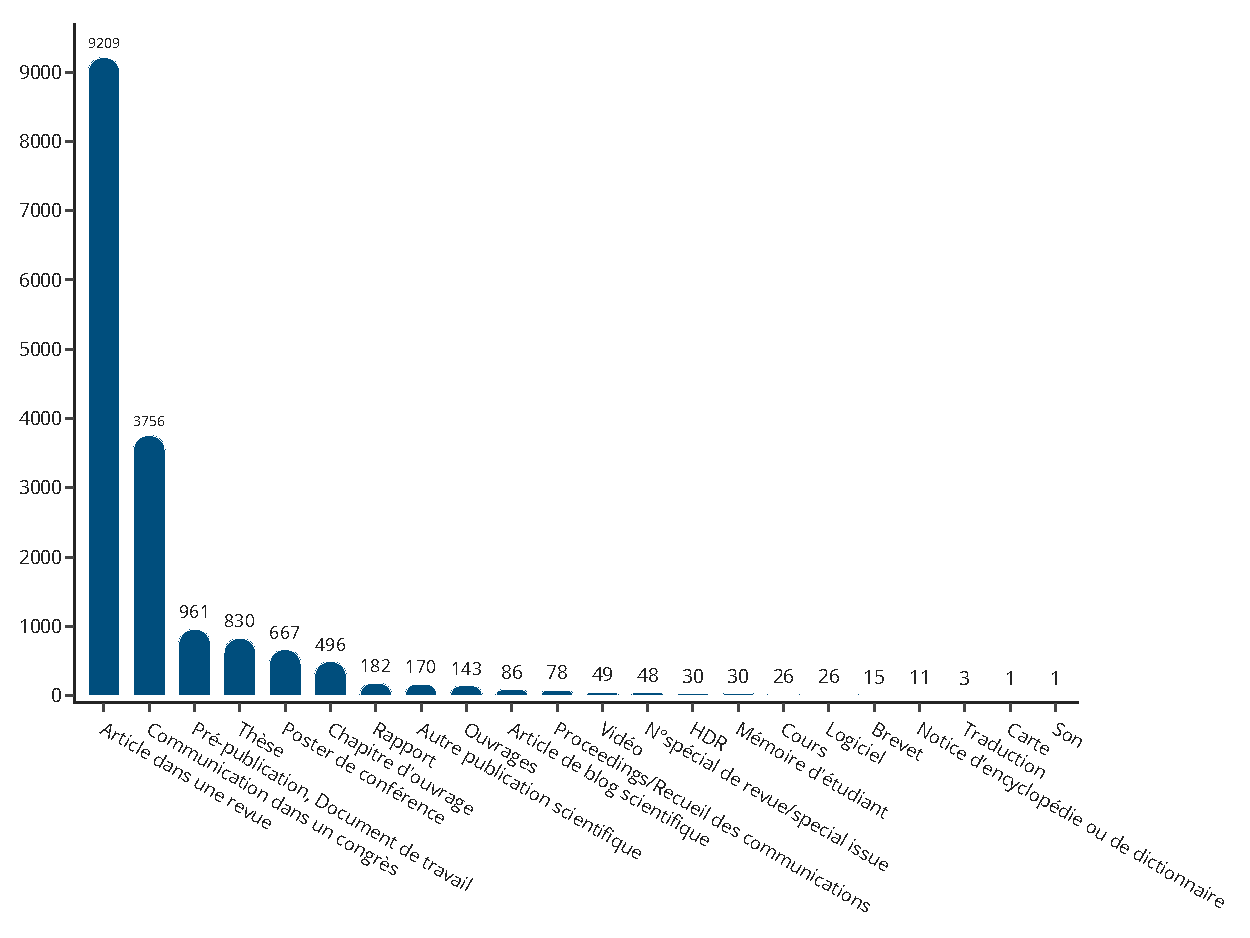
\includegraphics[width=\textwidth]{figures/works_type.pdf}
  \centering
  \caption{Types de documents renseignés dans HAL}
  \label{fig_doc_type}
\end{figure}

{\footnotesize\workstypeinfo}

% Ecrire un commentaire sur la typologie de la production scientifique ci-dessous :





% Fin de la typologie de la production scientifique

\pagebreak

\section{Articles et Communications de congrès en accès ouvert} % Evolution sur une période de 5 ans (2020-2024)

\begin{figure}[!h]
  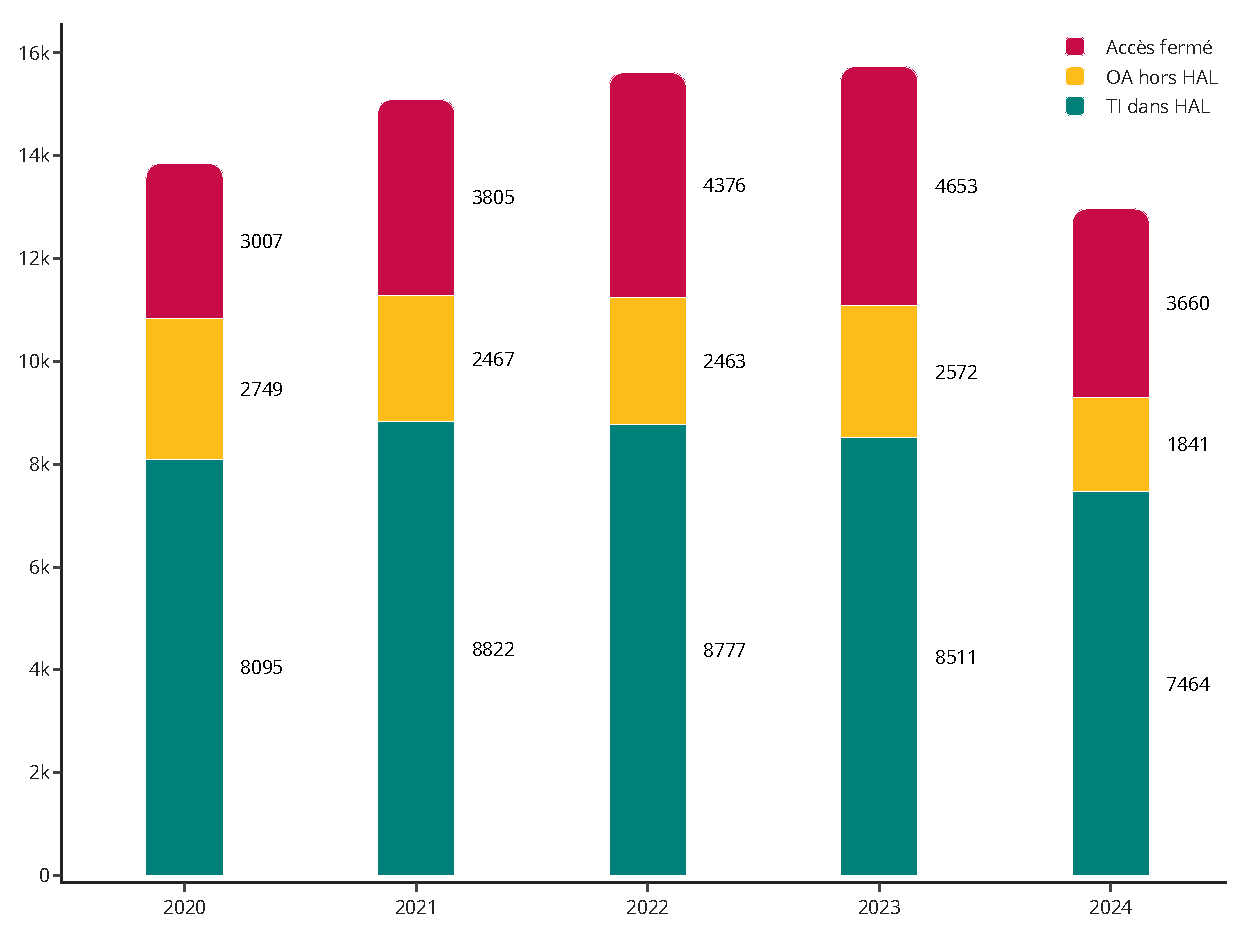
\includegraphics[width=\textwidth]{figures/open_access_works.pdf}
  \caption{Statut des accès ouverts des travaux sur la période {\oaworksperiod}}
  \label{fig_open_access_works}
\end{figure}

{\footnotesize\openaccessworksinfo}

\begin{tcolorbox}[colback=white, arc=4pt, boxrule=0.5pt, left=2pt, right=2pt, top=2pt, bottom=2pt]
\footnotesize
\begin{description}[leftmargin=!, labelwidth=\widthof{\bfseries OA Hors HAL}]
    \item[TI dans HAL] PDF librement accessible pour tous sur l'archive ouverte HAL
    \item[OA Hors HAL] PDF disponible sur les sites éditeurs, ou sur une archive ouverte autre que HAL, dépôt à l'étranger, disciplinaire tel que Arxiv, Pubmed etc
    \item[Accès fermé] notice seule sur HAL. En l'absence d'abonnement à la revue, les lecteurs n'ont pas accès au contenu.
\end{description}
\end{tcolorbox}

\bigskip

% Ecrire un commentaire sur les articles et communication de congrès en accès ouvert ci-dessous :





% Fin des articles et communication de congrès en accès ouvert

\pagebreak


\section[Version bêta]{Liste des revues et les voies d'accès ouvert repérés dans le BSO}

Ce tableau utilise des données du Baromètre français de la Science Ouverte. Ces données sont compilées le dernier trimestre de chaque année (généralement en décembre), sur les données de l'année précédente. Ainsi, le tableau montre le nombre de publications en accès ouvert lors du trimestre 2024Q4.

Il existe généralement un déficit de couverture d'environ 30 \% par rapport à HAL : sur {\bsojournalsnbworks} publications dans HAL, {\bsojournalsnbworksfoundinbso} ont été trouvées dans le BSO.

La colonne \say{APC payés} indique le montant de frais APC détecté comme payé par le BSO. Comme toute donnée collectée à travers de multiples sources hétérogènes, certaines données peuvent être manquantes ou inexactes, mais permettent néanmoins d'avoir un aperçu général de l'ouverture de la production scientifique.

{
  \footnotesize
  \begin{longtable}{p{.27\linewidth}P{.18\linewidth}P{.07\linewidth}P{.12\linewidth}P{.12\linewidth}P{.07\linewidth}}
\caption{Liste des revues, des éditeurs, des statuts d'accès ouvert et des APC payés. D'après la liste des publications dans HAL et les données du BSO 2024Q4.}
\label{tab_journals}\\
\toprule
Revue & Éditeur & Nombre de travaux & Est en accès ouvert sur le journal & Est en accès ouvert sur une archive & APC payés \\
\midrule
The European Physical Journal C & Springer Science and Business Media LLC & 28 & \emoji{check-mark-button} \emoji{check-mark-button} \emoji{check-mark-button} \emoji{check-mark-button} \emoji{check-mark-button} \emoji{check-mark-button} \emoji{check-mark-button} \emoji{check-mark-button} \emoji{check-mark-button} \emoji{check-mark-button} \emoji{check-mark-button} \emoji{check-mark-button} \emoji{check-mark-button} \emoji{check-mark-button} \emoji{check-mark-button} \emoji{check-mark-button} \emoji{check-mark-button} \emoji{check-mark-button} \emoji{check-mark-button} \emoji{check-mark-button} \emoji{check-mark-button} \emoji{check-mark-button} \emoji{check-mark-button} \emoji{check-mark-button} \emoji{check-mark-button} \emoji{check-mark-button} \emoji{check-mark-button} \emoji{check-mark-button} & \emoji{check-mark-button} \emoji{check-mark-button} \emoji{check-mark-button} \emoji{check-mark-button} \emoji{check-mark-button} \emoji{check-mark-button} \emoji{check-mark-button} \emoji{check-mark-button} \emoji{check-mark-button} \emoji{check-mark-button} \emoji{check-mark-button} \emoji{check-mark-button} \emoji{check-mark-button} \emoji{check-mark-button} \emoji{check-mark-button} \emoji{check-mark-button} \emoji{check-mark-button} \emoji{check-mark-button} \emoji{check-mark-button} \emoji{check-mark-button} \emoji{check-mark-button} \emoji{check-mark-button} \emoji{check-mark-button} \emoji{check-mark-button} \emoji{check-mark-button} \emoji{check-mark-button} \emoji{check-mark-button} \emoji{check-mark-button} &  \\
Physics Letters B & Elsevier BV & 22 & \emoji{check-mark-button} \emoji{check-mark-button} \emoji{check-mark-button} \emoji{check-mark-button} \emoji{check-mark-button} \emoji{check-mark-button} \emoji{check-mark-button} \emoji{check-mark-button} \emoji{check-mark-button} \emoji{check-mark-button} \emoji{check-mark-button} \emoji{check-mark-button} \emoji{check-mark-button} \emoji{check-mark-button} \emoji{check-mark-button} \emoji{check-mark-button} \emoji{check-mark-button} \emoji{check-mark-button} \emoji{check-mark-button} \emoji{check-mark-button} \emoji{check-mark-button} \emoji{check-mark-button} & \emoji{check-mark-button} \emoji{check-mark-button} \emoji{check-mark-button} \emoji{check-mark-button} \emoji{check-mark-button} \emoji{check-mark-button} \emoji{check-mark-button} \emoji{check-mark-button} \emoji{check-mark-button} \emoji{check-mark-button} \emoji{check-mark-button} \emoji{check-mark-button} \emoji{check-mark-button} \emoji{check-mark-button} \emoji{check-mark-button} \emoji{check-mark-button} \emoji{check-mark-button} \emoji{check-mark-button} \emoji{check-mark-button} \emoji{check-mark-button} \emoji{check-mark-button} \emoji{check-mark-button} &  \\
Monthly Notices of the Royal Astronomical Society & Oxford University Press (OUP) & 12 & \emoji{check-mark-button} \emoji{check-mark-button} \emoji{check-mark-button} \emoji{check-mark-button} \emoji{check-mark-button} \emoji{check-mark-button} \emoji{check-mark-button} \emoji{check-mark-button} \emoji{check-mark-button} \emoji{check-mark-button} \emoji{check-mark-button} \emoji{check-mark-button} & \emoji{check-mark-button} \emoji{check-mark-button} \emoji{check-mark-button} \emoji{check-mark-button} \emoji{check-mark-button} \emoji{check-mark-button} \emoji{check-mark-button} \emoji{check-mark-button} \emoji{check-mark-button} \emoji{check-mark-button} \emoji{check-mark-button} \emoji{check-mark-button} & 2310 £, 2310 £, 2310 £, 2310 £, 2310 £, 2310 £, 2310 £, 2310 £, 2310 £, 2310 £, 2310 £ \\
Journal of Cosmology and Astroparticle Physics & IOP Publishing & 12 & \emoji{check-mark-button} \emoji{check-mark-button} \emoji{white-question-mark} \emoji{white-question-mark} \emoji{white-question-mark} \emoji{check-mark-button} \emoji{white-question-mark} \emoji{check-mark-button} \emoji{white-question-mark} \emoji{check-mark-button} \emoji{white-question-mark} \emoji{check-mark-button} & \emoji{check-mark-button} \emoji{check-mark-button} \emoji{check-mark-button} \emoji{check-mark-button} \emoji{check-mark-button} \emoji{check-mark-button} \emoji{check-mark-button} \emoji{check-mark-button} \emoji{check-mark-button} \emoji{check-mark-button} \emoji{check-mark-button} \emoji{check-mark-button} &  \\
EPJ Web of Conferences & EDP Sciences & 11 & \emoji{check-mark-button} \emoji{check-mark-button} \emoji{check-mark-button} \emoji{check-mark-button} \emoji{check-mark-button} \emoji{check-mark-button} \emoji{check-mark-button} \emoji{check-mark-button} \emoji{check-mark-button} \emoji{check-mark-button} \emoji{check-mark-button} & \emoji{check-mark-button} \emoji{check-mark-button} \emoji{check-mark-button} \emoji{check-mark-button} \emoji{check-mark-button} \emoji{check-mark-button} \emoji{check-mark-button} \emoji{check-mark-button} \emoji{check-mark-button} \emoji{check-mark-button} \emoji{check-mark-button} &  \\
The European Physical Journal A & Springer Science and Business Media LLC & 10 & \emoji{white-question-mark} \emoji{check-mark-button} \emoji{check-mark-button} \emoji{white-question-mark} \emoji{check-mark-button} \emoji{white-question-mark} \emoji{check-mark-button} \emoji{white-question-mark} \emoji{check-mark-button} \emoji{white-question-mark} & \emoji{check-mark-button} \emoji{check-mark-button} \emoji{check-mark-button} \emoji{check-mark-button} \emoji{check-mark-button} \emoji{check-mark-button} \emoji{check-mark-button} \emoji{check-mark-button} \emoji{check-mark-button} \emoji{check-mark-button} & 2790 €, 2790 € \\
Automatica & Elsevier ; Elsevier BV & 7 & \emoji{white-question-mark} \emoji{white-question-mark} \emoji{white-question-mark} \emoji{white-question-mark} \emoji{cross-mark} \emoji{white-question-mark} \emoji{white-question-mark} & \emoji{check-mark-button} \emoji{check-mark-button} \emoji{check-mark-button} \emoji{check-mark-button} \emoji{white-question-mark} \emoji{check-mark-button} \emoji{check-mark-button} &  \\
Proceedings of 38th International Cosmic Ray Conference — PoS(ICRC2023) & Sissa Medialab & 7 & \emoji{check-mark-button} \emoji{check-mark-button} \emoji{check-mark-button} \emoji{check-mark-button} \emoji{check-mark-button} \emoji{check-mark-button} \emoji{check-mark-button} & \emoji{check-mark-button} \emoji{check-mark-button} \emoji{check-mark-button} \emoji{check-mark-button} \emoji{check-mark-button} \emoji{check-mark-button} \emoji{check-mark-button} &  \\
Journal of Physics: Conference Series & IOP Publishing & 6 & \emoji{check-mark-button} \emoji{check-mark-button} \emoji{check-mark-button} \emoji{check-mark-button} \emoji{check-mark-button} \emoji{check-mark-button} & \emoji{check-mark-button} \emoji{check-mark-button} \emoji{check-mark-button} \emoji{check-mark-button} \emoji{check-mark-button} \emoji{check-mark-button} &  \\
Nuclear Instruments and Methods in Physics Research Section A Accelerators Spectrometers Detectors and Associated Equipment & Elsevier BV & 5 & \emoji{white-question-mark} \emoji{check-mark-button} \emoji{cross-mark} \emoji{cross-mark} \emoji{cross-mark} & \emoji{check-mark-button} \emoji{check-mark-button} \emoji{white-question-mark} \emoji{white-question-mark} \emoji{white-question-mark} & 2690 \$ \\
Lecture notes in computer science & Springer Nature Switzerland & 5 & \emoji{cross-mark} \emoji{white-question-mark} \emoji{cross-mark} \emoji{cross-mark} \emoji{cross-mark} & \emoji{white-question-mark} \emoji{check-mark-button} \emoji{white-question-mark} \emoji{white-question-mark} \emoji{white-question-mark} &  \\
The Astrophysical Journal & American Astronomical Society & 4 & \emoji{check-mark-button} \emoji{check-mark-button} \emoji{check-mark-button} \emoji{check-mark-button} & \emoji{check-mark-button} \emoji{check-mark-button} \emoji{check-mark-button} \emoji{check-mark-button} & 4499 \$, 4499 \$, 4499 \$, 4499 \$ \\
Journal of Cleaner Production & Elsevier BV & 4 & \emoji{cross-mark} \emoji{check-mark-button} \emoji{white-question-mark} \emoji{check-mark-button} & \emoji{white-question-mark} \emoji{check-mark-button} \emoji{check-mark-button} \emoji{check-mark-button} & 4100 \$, 4100 \$ \\
Communications Earth \& Environment & Springer Science and Business Media LLC & 4 & \emoji{check-mark-button} \emoji{check-mark-button} \emoji{check-mark-button} \emoji{check-mark-button} & \emoji{check-mark-button} \emoji{check-mark-button} \emoji{check-mark-button} \emoji{check-mark-button} & 1990 £, 1990 £, 1990 £, 1990 £ \\
International Journal of Production Research & Informa UK Limited & 4 & \emoji{cross-mark} \emoji{cross-mark} \emoji{cross-mark} \emoji{white-question-mark} & \emoji{white-question-mark} \emoji{white-question-mark} \emoji{white-question-mark} \emoji{check-mark-button} &  \\
Journal of Physics A Mathematical and Theoretical & IOP Publishing & 4 & \emoji{check-mark-button} \emoji{check-mark-button} \emoji{check-mark-button} \emoji{white-question-mark} & \emoji{check-mark-button} \emoji{check-mark-button} \emoji{check-mark-button} \emoji{check-mark-button} &  \\
Proceedings of The European Physical Society Conference on High Energy Physics — PoS(EPS-HEP2023) & Sissa Medialab & 4 & \emoji{check-mark-button} \emoji{check-mark-button} \emoji{check-mark-button} \emoji{check-mark-button} & \emoji{check-mark-button} \emoji{check-mark-button} \emoji{check-mark-button} \emoji{check-mark-button} &  \\
Systems \& Control Letters & Elsevier BV & 4 & \emoji{white-question-mark} \emoji{white-question-mark} \emoji{white-question-mark} \emoji{white-question-mark} & \emoji{check-mark-button} \emoji{check-mark-button} \emoji{check-mark-button} \emoji{check-mark-button} &  \\
The Science of The Total Environment & Elsevier BV & 4 & \emoji{cross-mark} \emoji{cross-mark} \emoji{cross-mark} \emoji{cross-mark} & \emoji{white-question-mark} \emoji{white-question-mark} \emoji{white-question-mark} \emoji{white-question-mark} &  \\
Pest Management Science & Wiley & 3 & \emoji{check-mark-button} \emoji{white-question-mark} \emoji{cross-mark} & \emoji{check-mark-button} \emoji{check-mark-button} \emoji{white-question-mark} & 5100 \$ \\
Global Change Biology & Wiley & 3 & \emoji{cross-mark} \emoji{check-mark-button} \emoji{check-mark-button} & \emoji{white-question-mark} \emoji{check-mark-button} \emoji{check-mark-button} & 4120 \$, 4120 \$ \\
Icarus & Elsevier BV & 3 & \emoji{cross-mark} \emoji{white-question-mark} \emoji{check-mark-button} & \emoji{white-question-mark} \emoji{check-mark-button} \emoji{check-mark-button} & 3590 \$ \\
Meteoritics and Planetary Science & Wiley & 3 & \emoji{white-question-mark} \emoji{check-mark-button} \emoji{check-mark-button} & \emoji{check-mark-button} \emoji{check-mark-button} \emoji{check-mark-button} & 3090 \$, 3090 \$ \\
International Journal of Molecular Sciences & MDPI AG & 3 & \emoji{check-mark-button} \emoji{check-mark-button} \emoji{check-mark-button} & \emoji{check-mark-button} \emoji{check-mark-button} \emoji{check-mark-button} & 2300 CHF, 2300 CHF, 2300 CHF \\
Annales Henri Poincaré & Springer Science and Business Media LLC & 3 & \emoji{white-question-mark} \emoji{check-mark-button} \emoji{white-question-mark} & \emoji{check-mark-button} \emoji{check-mark-button} \emoji{check-mark-button} & 2290 € \\
\textbf{Seulement 25 lignes affichées sur 501.} \\
\bottomrule
\end{longtable}

}

{\footnotesize\journalsinfo}

\pagebreak

\section{Carte des collaborations internationales}

{\collaborationsnb} collaborations parmi {\institutionsnb} institutions dans {\countriesnb} pays.

\begin{figure}[!h]
  \hspace{-.1\textwidth}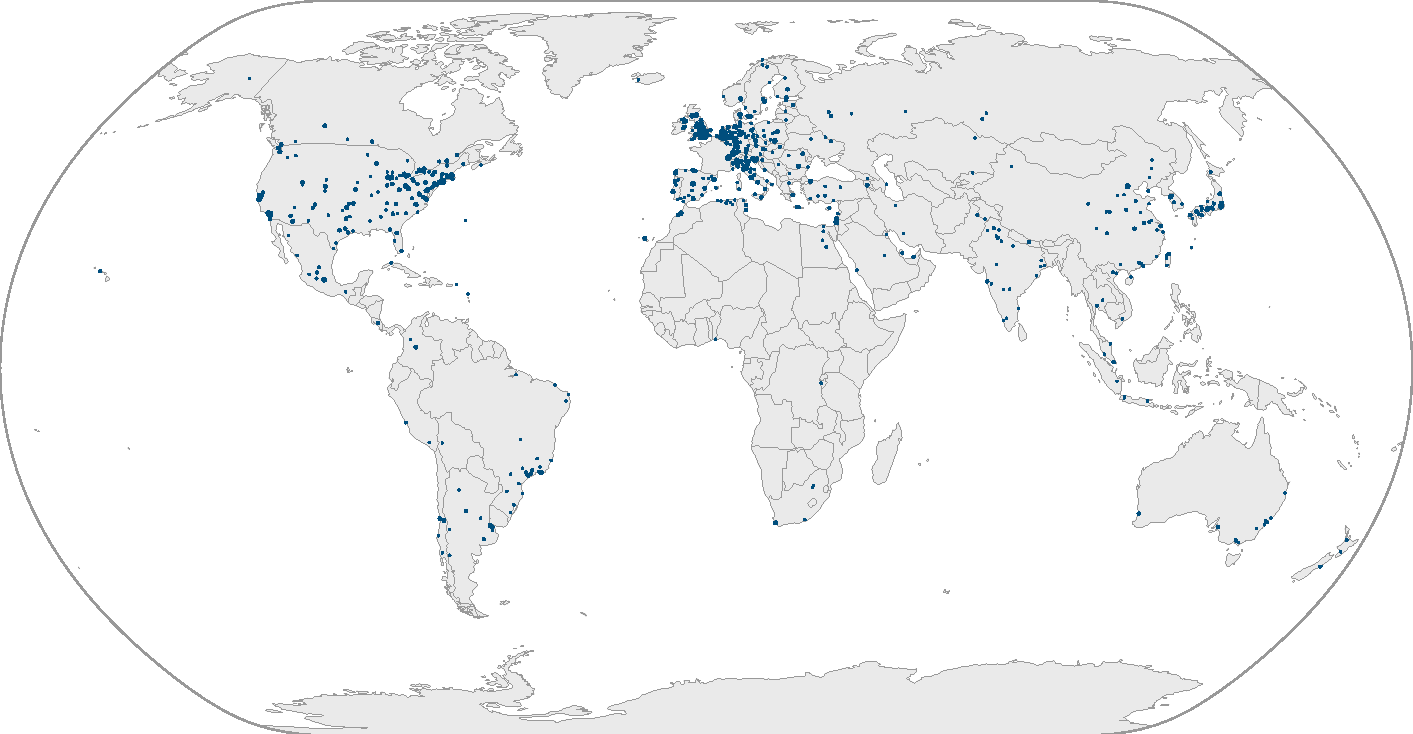
\includegraphics[width=1.2\textwidth]{figures/collaboration_map_world.pdf}
  \caption{Collaborations Internationales - Données : publications renseignées dans HAL avec un DOI, en utilisant les métadonnées d'OpenAlex}
  \label{fig_collab_map}
\end{figure}

{\footnotesize\collaborationmapworldinfo}

\pagebreak

\section{Carte des collaborations Européennes}

\begin{figure}[!h]
  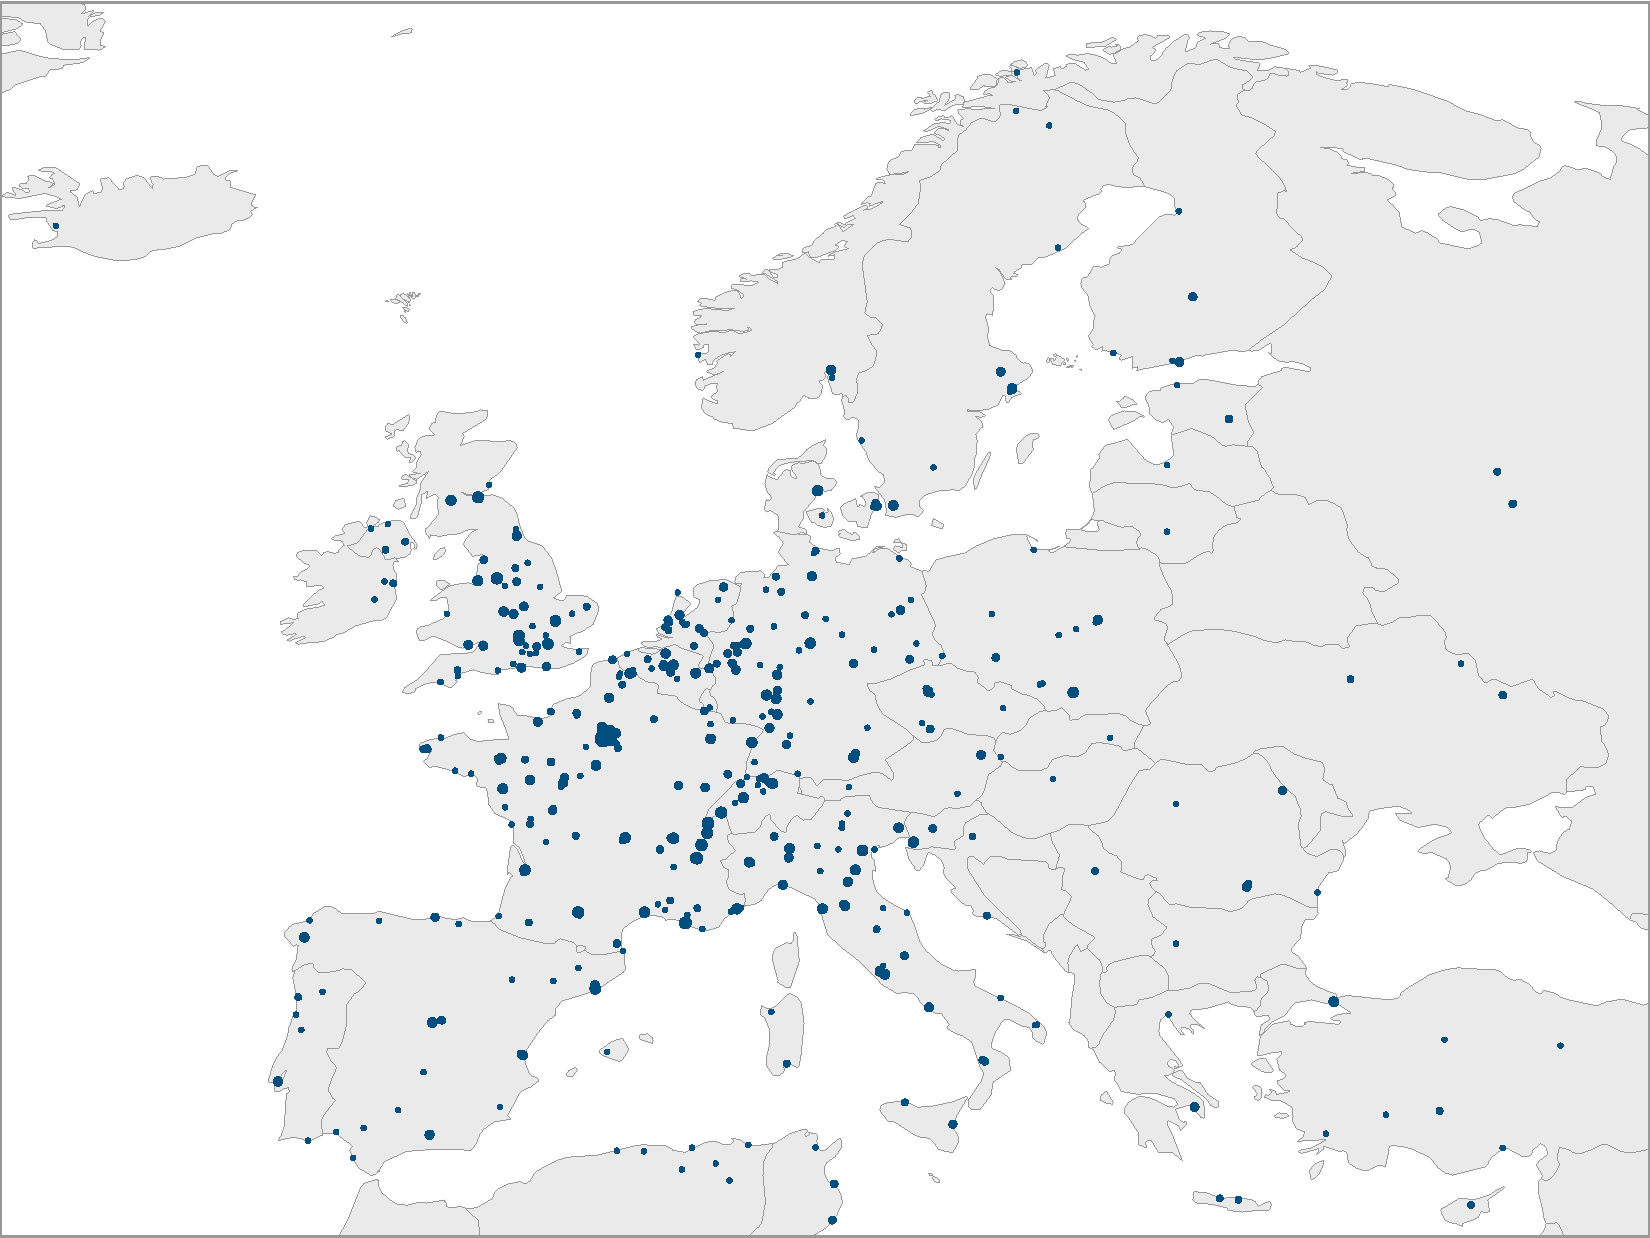
\includegraphics[width=\textwidth]{figures/collaboration_map_europe.pdf}
  \caption{Collaborations Européennes - Données : publications renseignées dans HAL avec un DOI, en utilisant les métadonnées d'OpenAlex}
  \label{fig_collab_map_europe}
\end{figure}

{\footnotesize\collaborationmapeuropeinfo}

\pagebreak

\section{Collaborations internationales par établissements}

\begin{figure}[!h]
  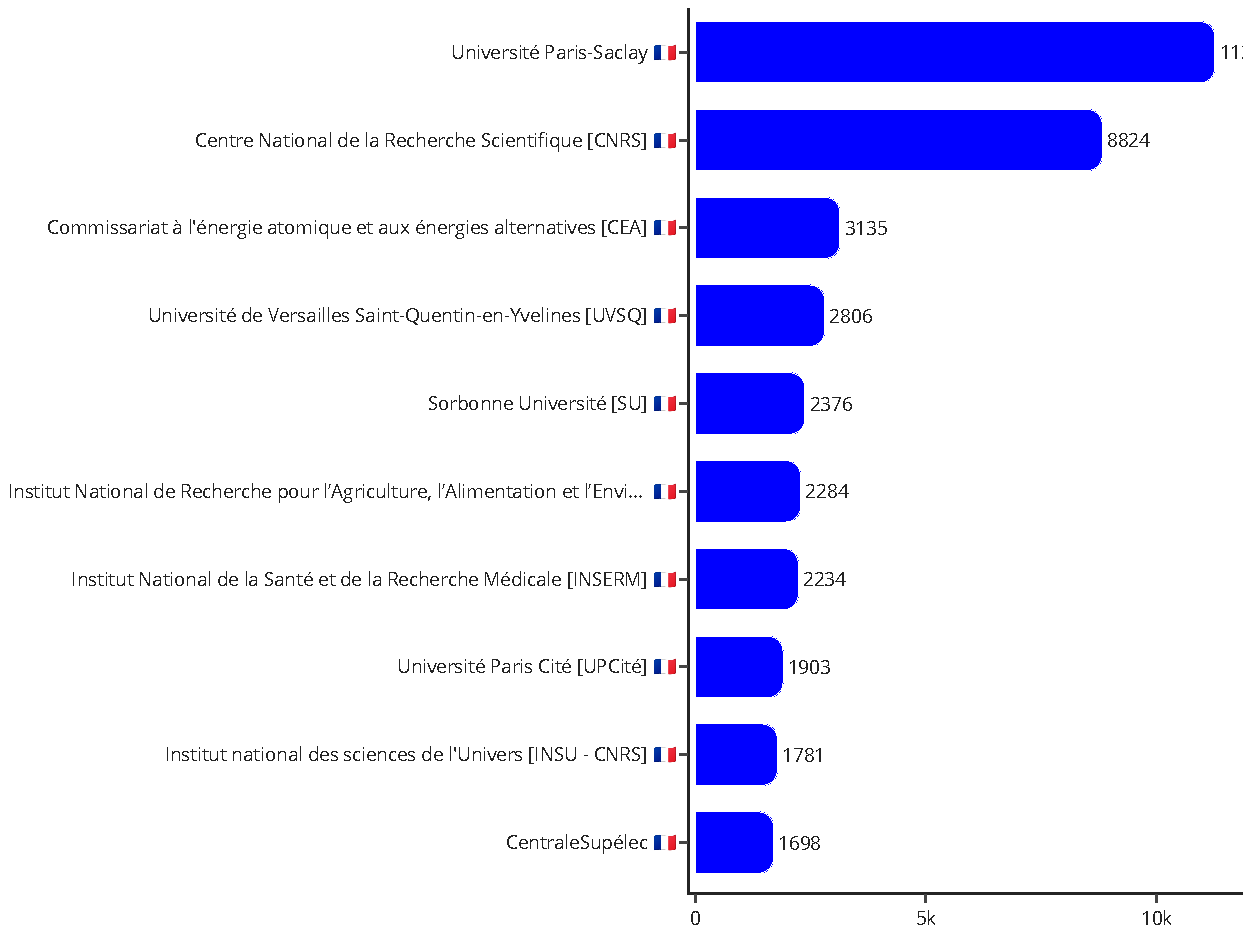
\includegraphics[width=\textwidth]{figures/collaboration_names.pdf}
  \caption{Collaborations internationales hors France - Données : Nom des institutions renseignées dans HAL}
  \label{fig_collab_names}
\end{figure}

{\footnotesize\collaborationnamesinfo}

\pagebreak

\section[Version bêta]{Collaborations (non académique) avec le secteur privé}

\begin{figure}[!h]
  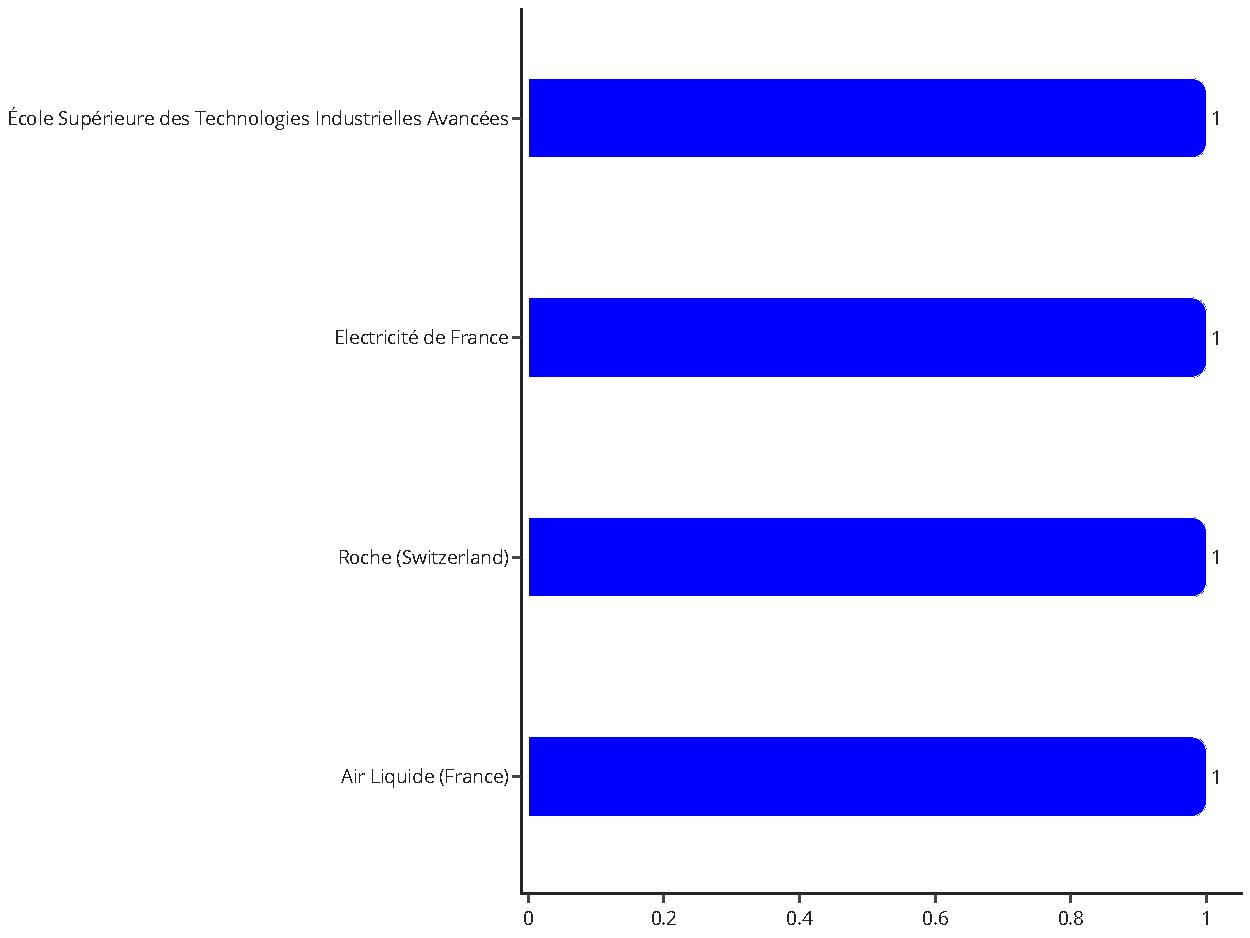
\includegraphics[width=\textwidth]{figures/private_sector_collaborations.pdf}
  \centering
  \caption{Collaborations avec le secteur privé - Données : publications renseignées dans HAL, en utilisant les métadonnées de scanR}
  \label{fig_private_collab}
\end{figure}

{\footnotesize\privatesectorcollaborationsinfo}


% Ecrire un commentaire sur les collaborations (non académique) avec le secteur privé  ci-dessous :





% Fin des collaborations (non académique) avec le secteur privé

\pagebreak

\section{Publications liées à des projets européens}

\begin{figure}[!h]
  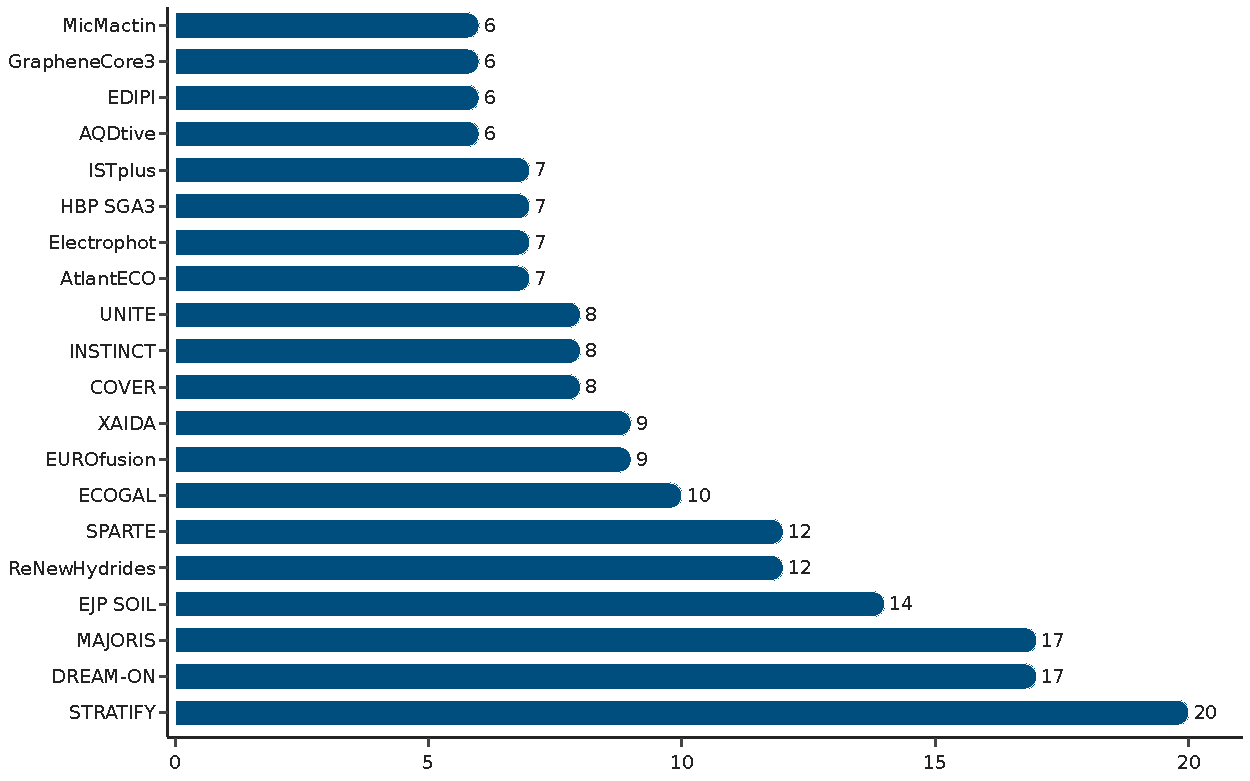
\includegraphics[width=.85\textwidth]{figures/european_projects.pdf}
  \centering
  \caption{Projets Européens renseignés dans HAL}
  \label{fig_eu_projects}
\end{figure}

{\footnotesize\europeanprojectsinfo}

\section{Publications liées à des projets ANR}

\begin{figure}[!h]
  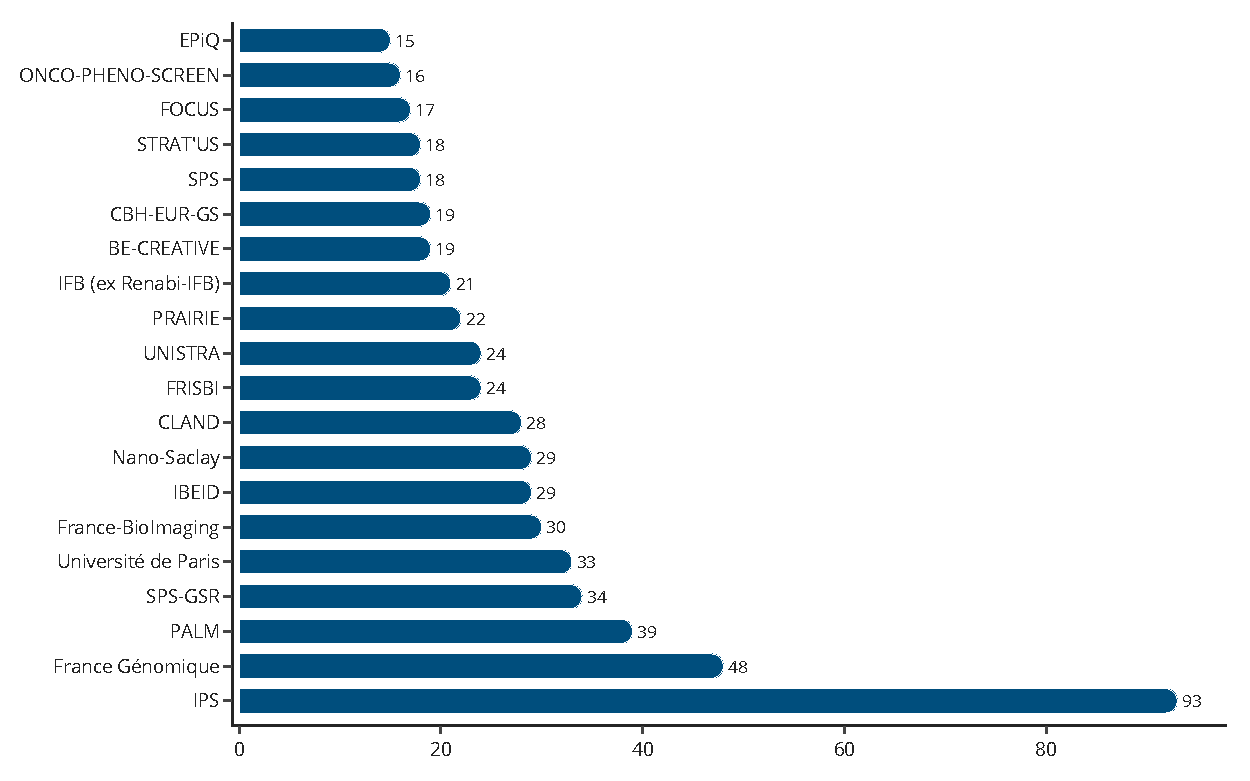
\includegraphics[width=.85\textwidth]{figures/anr_projects.pdf}
  \centering
  \caption{Projets ANR renseignés dans HAL}
  \label{fig_anr_projects}
\end{figure}

{\footnotesize\anrprojectsinfo}

\pagebreak

\section{Données – jeux de données partagés}

% Ecrire un commentaire sur les données - jeux de données partagés ci-dessous :





% Fin des données - jeux de données partagés

\pagebreak

\section{Les atouts du Laboratoire dans son engagement pour la science ouverte}

% Ecrire un commentaire sur les atouts du Laboratoire dans son engagement pour la science ouverte ci-dessous :





% Fin des atouts du Laboratoire dans son engagement pour la science ouverte 


\section{Préconisations, pour aller plus loin}

% Ecrire un commentaire sur les préconisations, pour aller plus loin ci-dessous :





% Fin des préconisations, pour aller plus loin


\vfill

\paragraph{Rappel :} la loi pour la République Numérique permet aux auteurs travaillant dans une institution publique en France depuis 2016, de partager le postprint sur HAL, avec un embargo de 6 mois pour les disciplines STM et 1 an pour les SHS.


\makelastpagereport
 
\end{document}
